\documentclass[document.tex]{subfiles}
\begin{document}
\chapter{Wyniki badań doświadczalnych \\ implementacji algorytmu Viterbiego}
\indent Do określenia poprawności działania opracowanej metody detekcji linii, 
wykorzystano zdjęcia z różnym poziomem zaszumienia. W celu porównania szybkości
działania poszczególnych implementacji algorytmu zdefiniowano zestaw zdjęć testowych
o różnym rozmiarze. Do przedstawienia wyników zestawień parametrów algorytmu Viterbiego
dla różnych wersji implementacji, została napisana funkcja automatycznie generująca plik .csv,
zawierający tabelę z parametrami wejściowymi oraz zestawienie szybkości przetwarzania każdego zdjęcia.
Na podstawie otrzymanego pliku zostały stworzone wykresy wizualizujące i umożliwiające
analizę i wyciągnięcie wniosków z przeprowadzonych badań.

%wrzucić zdjęcia pokazujące przykładowe wyniki detekcji linii dla różnych rodzajów obrazu - 3
%zdjęcia z przed i po
\begin{figure}[h]
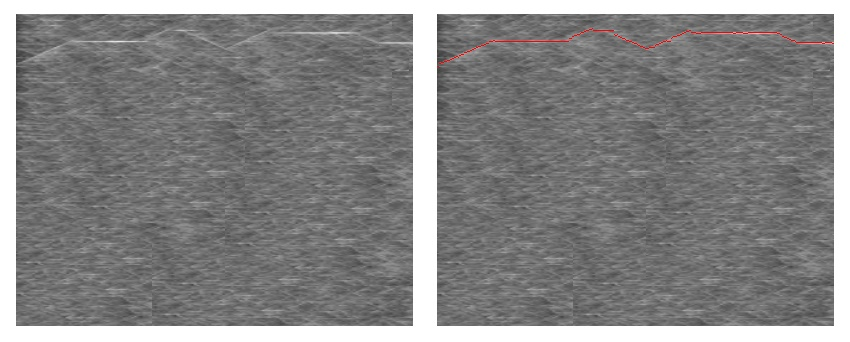
\includegraphics[scale=0.05]{detect_diff_0}
\caption{Przykład detekcji linii za pomocą algorytmu przedstawionego w rozdziale \ref{viterbi_line}}
\label{fig:sample_detect_0}
\end{figure}

\clearpage

\begin{figure}[h]
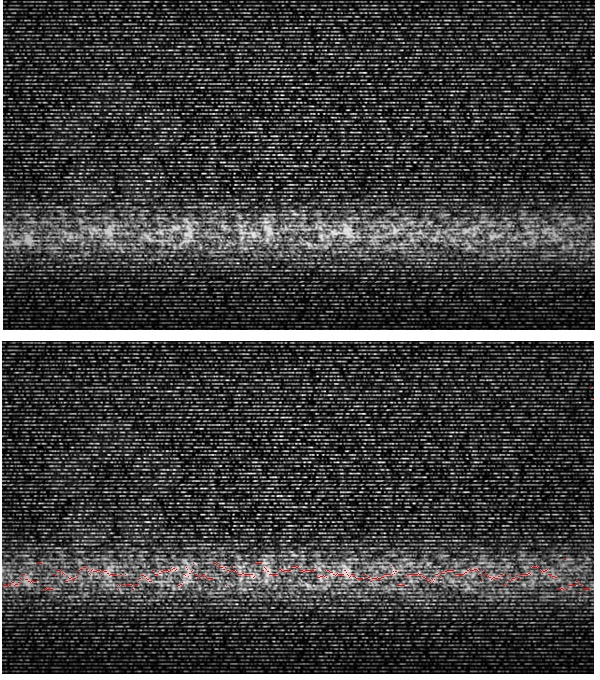
\includegraphics[scale=0.05]{detect_diff_1}
\caption{Przykład detekcji linii za pomocą algorytmu przedstawionego w rozdziale \ref{viterbi_line}}
\label{fig:sample_detect_1}
\end{figure}

\section{Porównanie czasu działania dla implementacji szeregowej, wielowątkowej
oraz z wykorzystaniem biblioteki OpenCL}
\indent W celu przetestowania szybkości opracowanego algorytmu wykorzystującego
kartę graficzną, porównano go z czterema innymi implementacjami algorytmu Viterbiego opisanymi
w rozdziale \ref{viterbi_chapter}.
W celu bardziej wymagającej oceny implementacji na GPU względem algorytmów wykorzystujących CPU, dodano
do flag kompilatora opcję \code{-O2} w celu włączenia optymalizacji kodu programu.
Dzięki temu zaobserwowano diametralny wzrost szybkości wykonywania tych algorytmów.
\\
\indent Algorytmy były porównywane na podstawie szybkości przetwarzania zdjęć
w zależności od ich rozmiaru oraz zakresu lokalnego sąsiedztwa $g\in \langle g_l, g_h \rangle$
(patrz rozdział \ref{viterbi_line}). Od niego zależała dokładność wykrycia linii, 
jeśli został dobrany zbyt mały zakres $g$ linia nie była wykrywana poprawnie jeśli, 
występowały większe jej kierunku(patrz rys.\ref{fig:g_range_results}). Dokładność wyznaczenia położenia linii
została przedstawiona wskaźnikiem błędu skumulowanego:

\begin{equation}
   Ec = \sum_{i=0}^{width - 1} |l_i - r_i|
    \label{eq:total_error}
\end{equation}
\myequations{Skumulowany błąd wyznaczenia położenia linii algorytmem Viterbiego}

, gdzie $r_i$ to i-ta współrzędna linii będąca wynikiem zastosowania algorytmu Viterbiego, 
\\$l_i$: i-ta rzeczywista współrzędna linii na obrazie, $Ec$ - błąd całkowity, 
$width$: szerokość zdjecia.

\begin{figure}[h]
\includegraphics[scale=0.045]{imgs/g_range_results.jpg}
\caption{Porównanie dokładności wykrycia linii dla \textbf{A} $g\in \langle -1, 1 \rangle$ i 
\textbf{B} $g\in \langle -6, 6 \rangle$}
\label{fig:g_range_results}
\end{figure}

\clearpage
\subsection{Zestawienie wynikow dla konfiguracji sprzętowej 
Intel i7-4790 4GHz, NVIDIA GeForce GTX 960}


%tabela z wynikami pc----------------------------------------------
\begin{figure}[h]
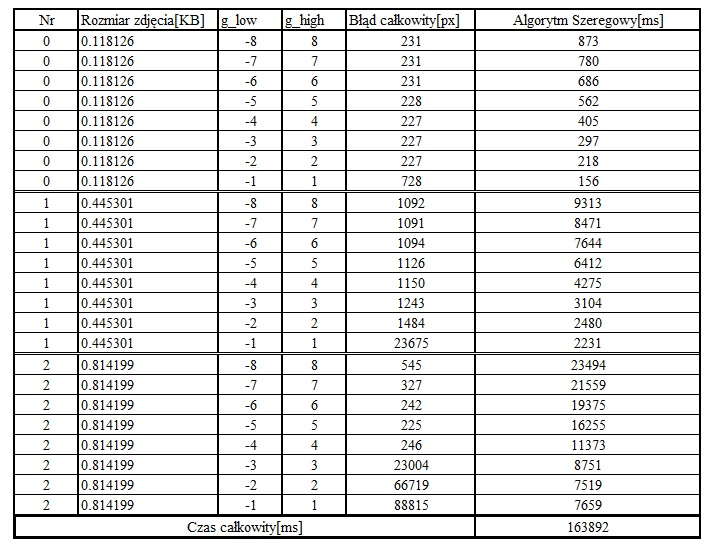
\includegraphics[scale=0.75]{imgs/results_pc_serial}
\caption{Wyniki badań dla algorytmu szeregowego}
\label{fig:results_pc_serial}
\end{figure}

\begin{figure}[h]
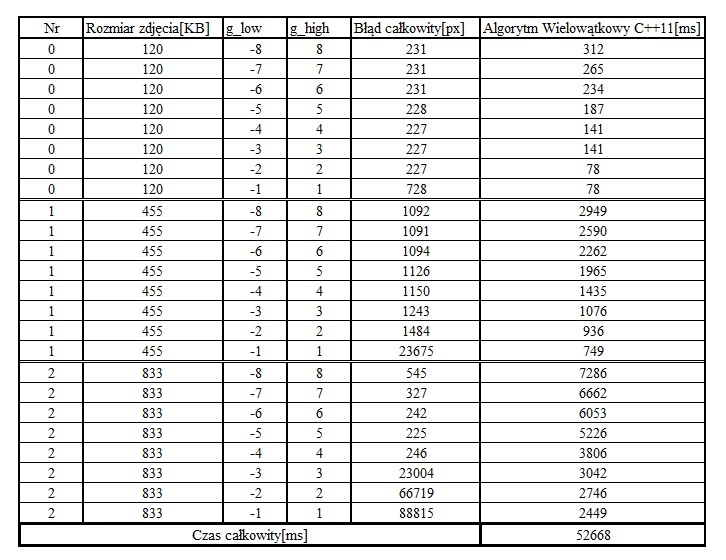
\includegraphics[scale=0.75]{imgs/results_pc_cpp11_threads.jpg}
\caption{Wyniki badań dla algorytmu wielowątkowego korzystającego z C++11}
\label{fig:results_pc_cpp11_threads}
\end{figure}

\begin{figure}[h]
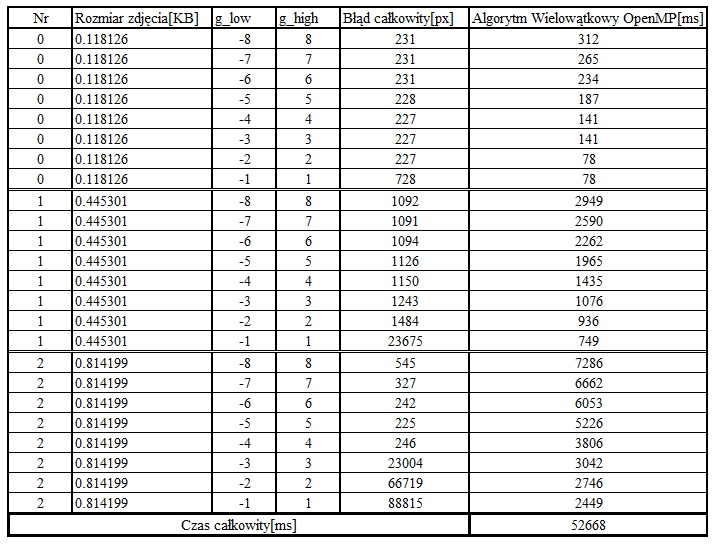
\includegraphics[scale=0.75]{imgs/results_pc_openmp_threads.jpg}
\caption{Wyniki badań dla algorytmu wielowątkowego OpenMP}
\label{fig:results_pc_openmp_threads}
\end{figure}

\begin{figure}[h]
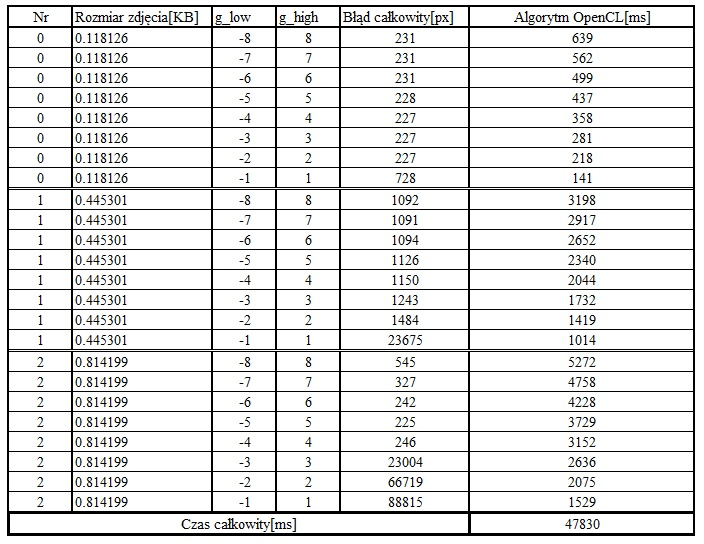
\includegraphics[scale=0.75]{imgs/results_pc_gpu.jpg}
\caption{Wyniki badań dla algorytmu OpenCL}
\label{fig:results_pc_gpu}
\end{figure}

\begin{figure}[h]
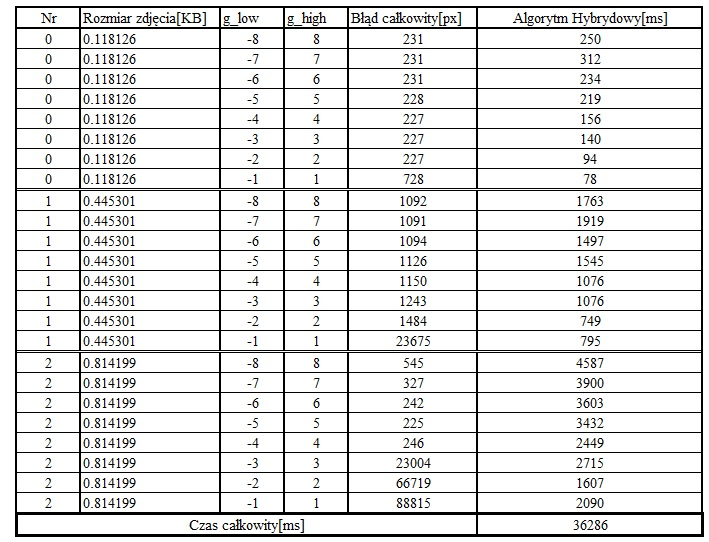
\includegraphics[scale=0.75]{imgs/results_pc_hybrid.jpg}
\caption{Wyniki badań dla algorytmu hybrydowego}
\label{fig:results_pc_hybrid}
\end{figure}

%--------------------------------------------------------------

%wykresy--------------------------------------------------------
\begin{figure}[h]
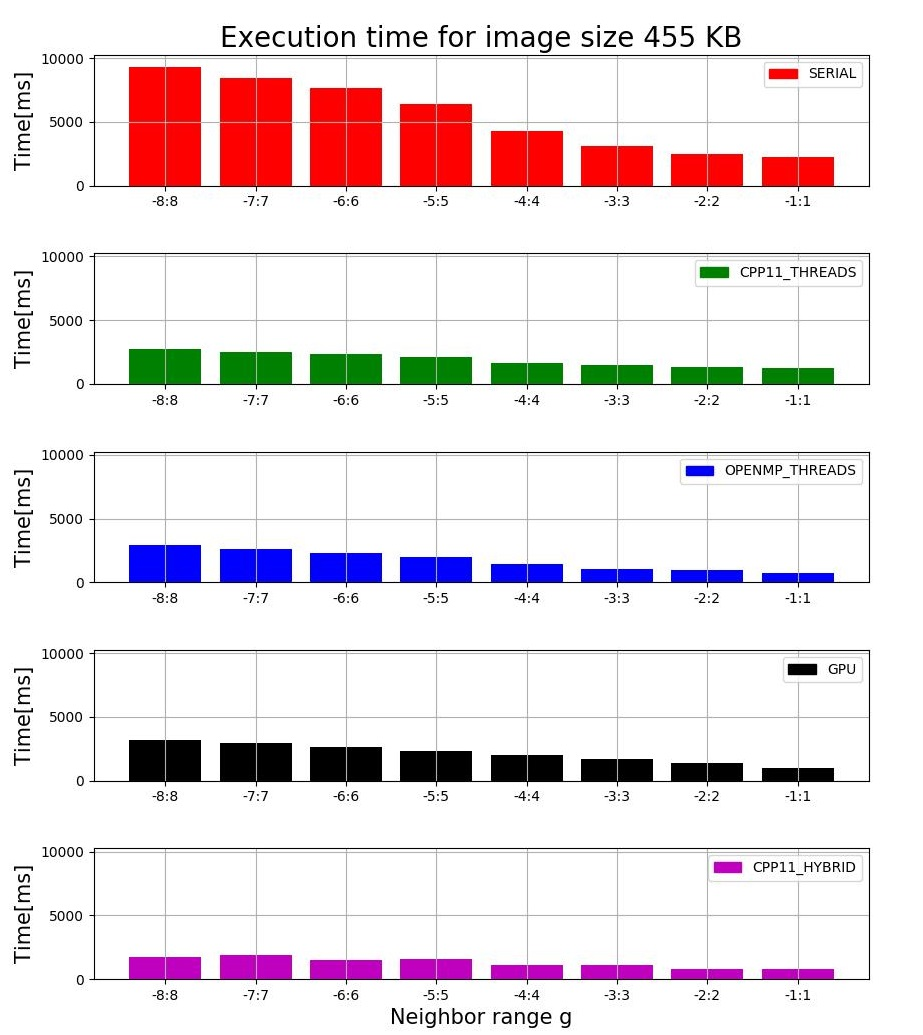
\includegraphics[scale=0.85]{imgs/plot0_pc.png}
\caption*{}
\label{fig:results_pc_hybrid}
\end{figure}

%wykresy
\begin{figure}[h]
\includegraphics[scale=0.85]{imgs/plot7_pc.png}
\caption{Zestawienie czasu wykonania algorytmów dla zdjęcia o rozmiarze 120kB, 
        w zależności od zakresu sąsiedztwa $g\in \langle -8, 8 \rangle$ : $g\in \langle -1, 1 \rangle$ }
\label{fig:results_pc_hybrid}
\end{figure}

%wykresy
\begin{figure}[h]
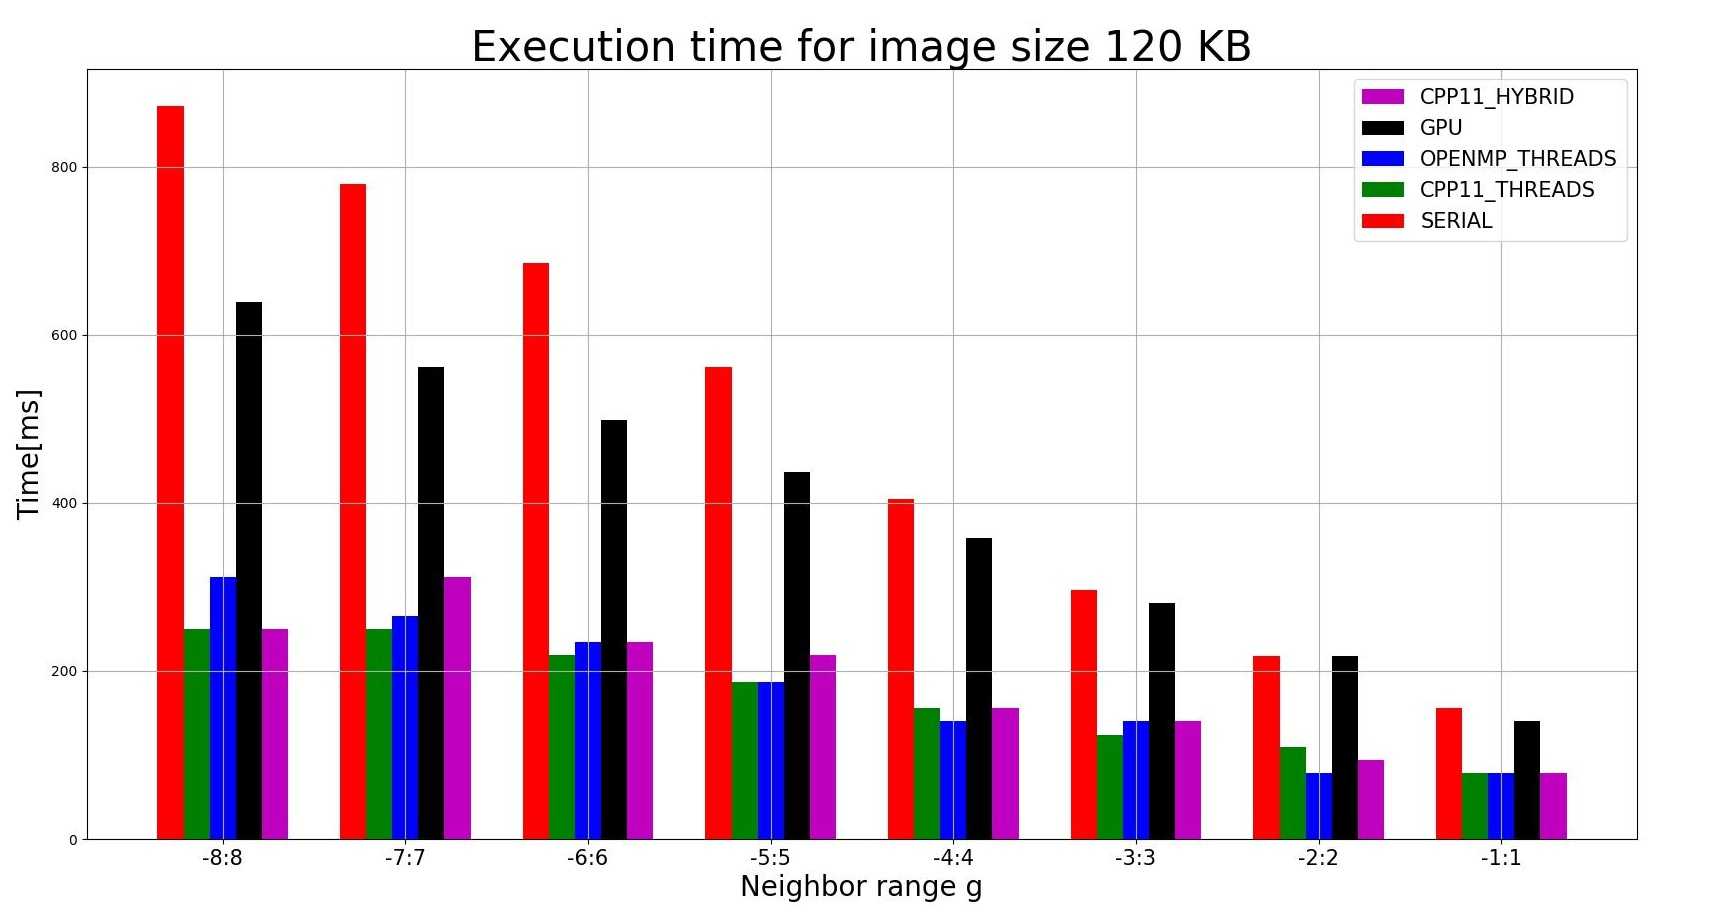
\includegraphics[scale=0.85]{imgs/plot5_pc.png}
\caption*{}
\label{fig:results_pc_hybrid}
\end{figure}

%wykresy
\begin{figure}[h]
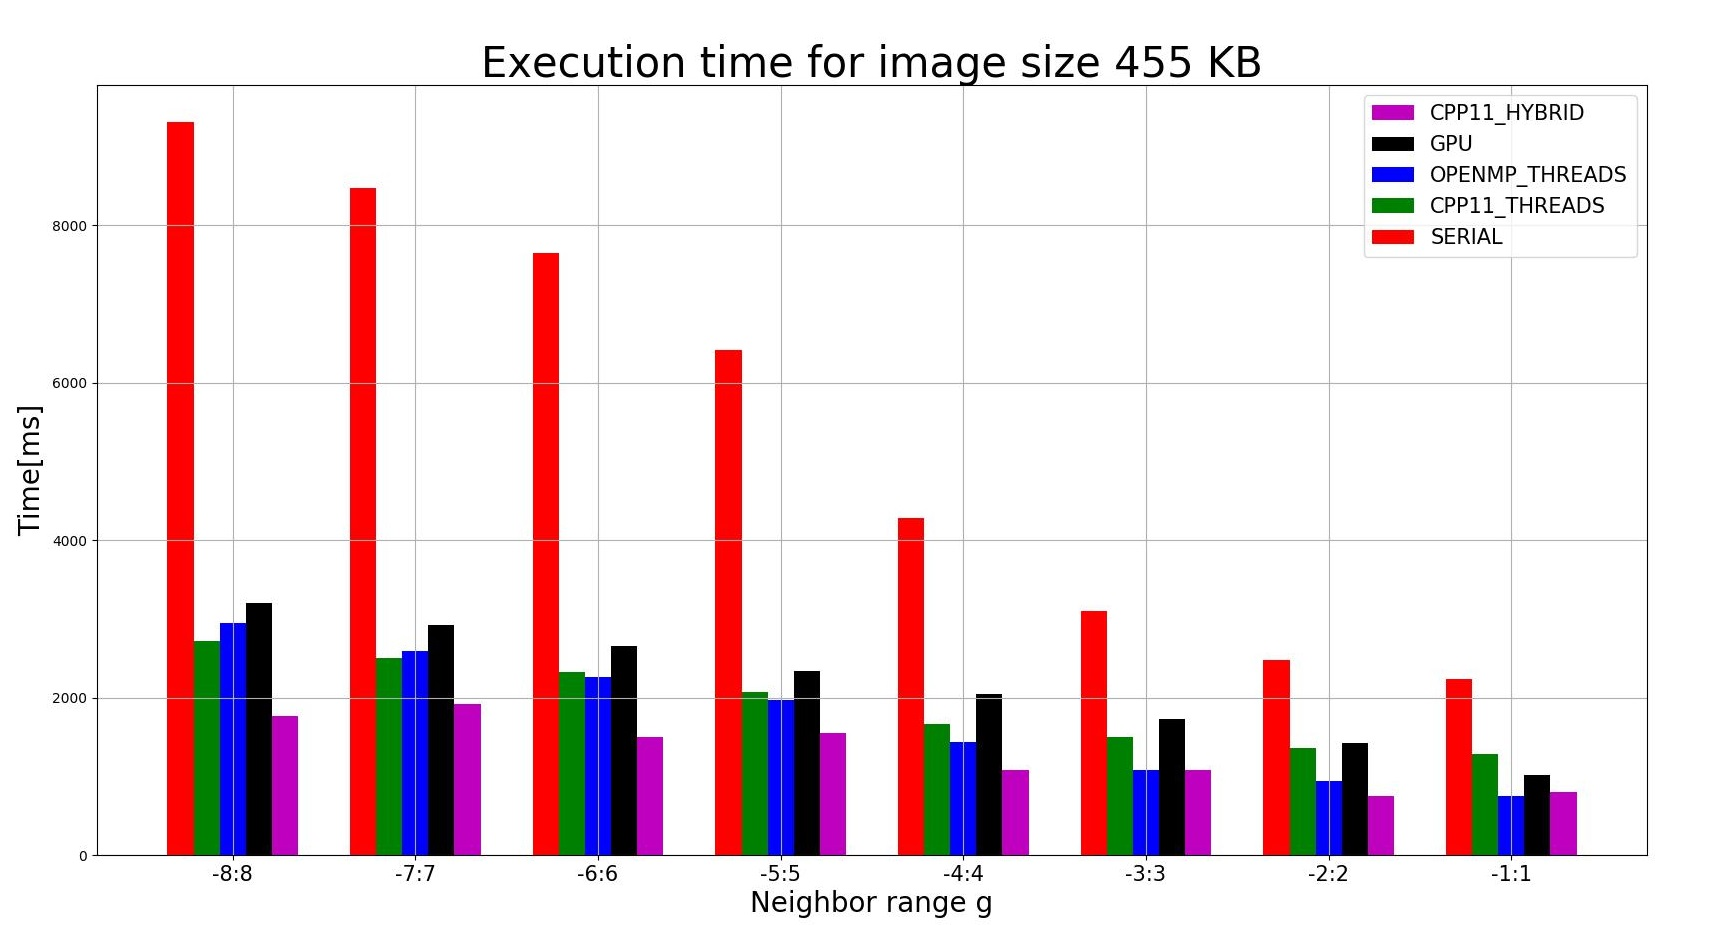
\includegraphics[scale=0.85]{imgs/plot4_pc.png}
\caption{Zestawienie czasu wykonania algorytmów dla zdjęcia o rozmiarze 455kB, 
        w zależności od zakresu sąsiedztwa $g\in \langle -8, 8 \rangle$ : $g\in \langle -1, 1 \rangle$ }
\label{fig:results_pc_hybrid}
\end{figure}

%wykresy
\begin{figure}[h]
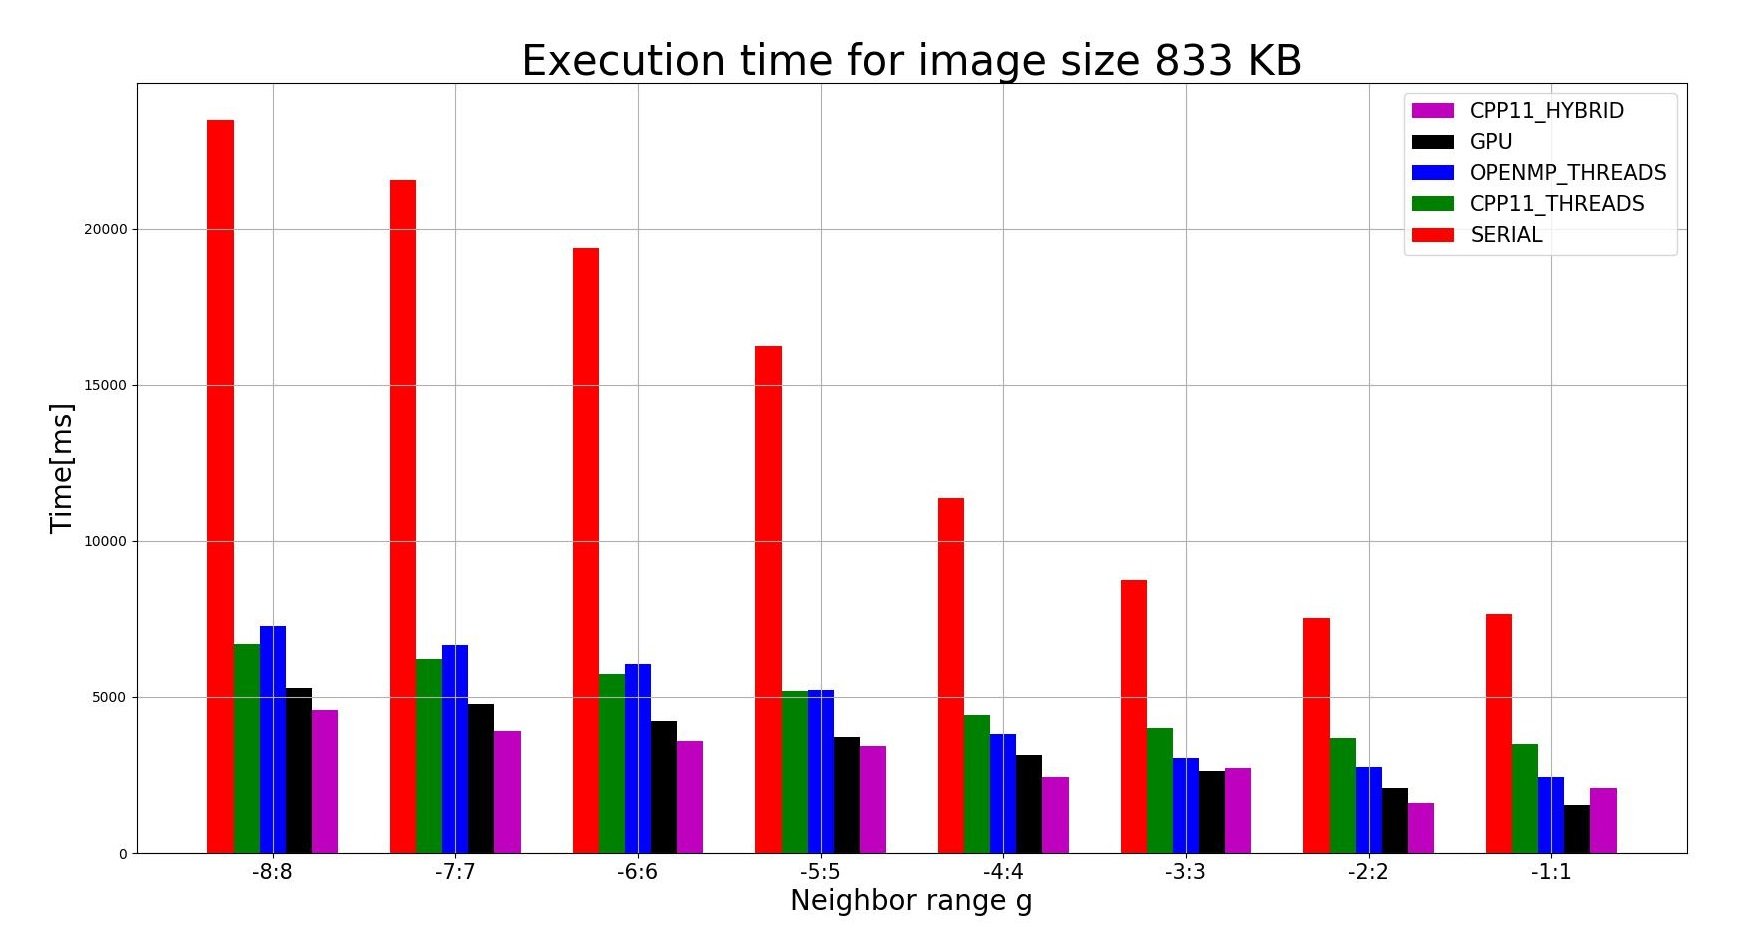
\includegraphics[scale=0.85]{imgs/plot6_pc.png}
\caption*{}
\label{fig:results_pc_hybrid}
\end{figure}

%wykresy
\begin{figure}[h]
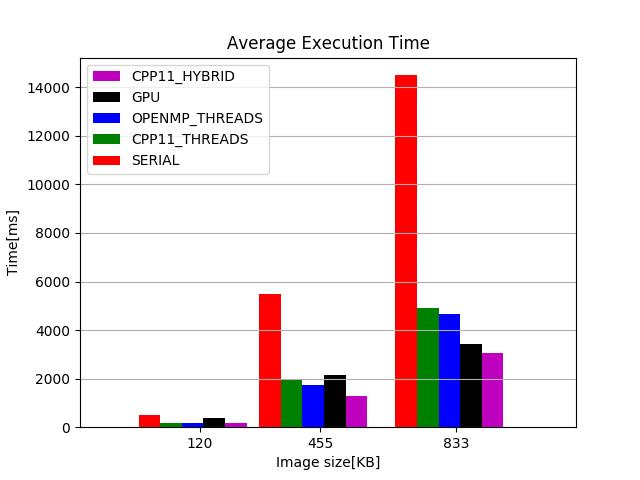
\includegraphics[scale=0.85]{imgs/plot1_pc.png}
\caption{Zestawienie czasu wykonania algorytmów dla zdjęcia o rozmiarze 833kB, 
        w zależności od zakresu sąsiedztwa $g\in \langle -8, 8 \rangle$ : $g\in \langle -1, 1 \rangle$ }
\label{fig:results_pc_hybrid}
\end{figure}

%wykresy
\begin{figure}[h]
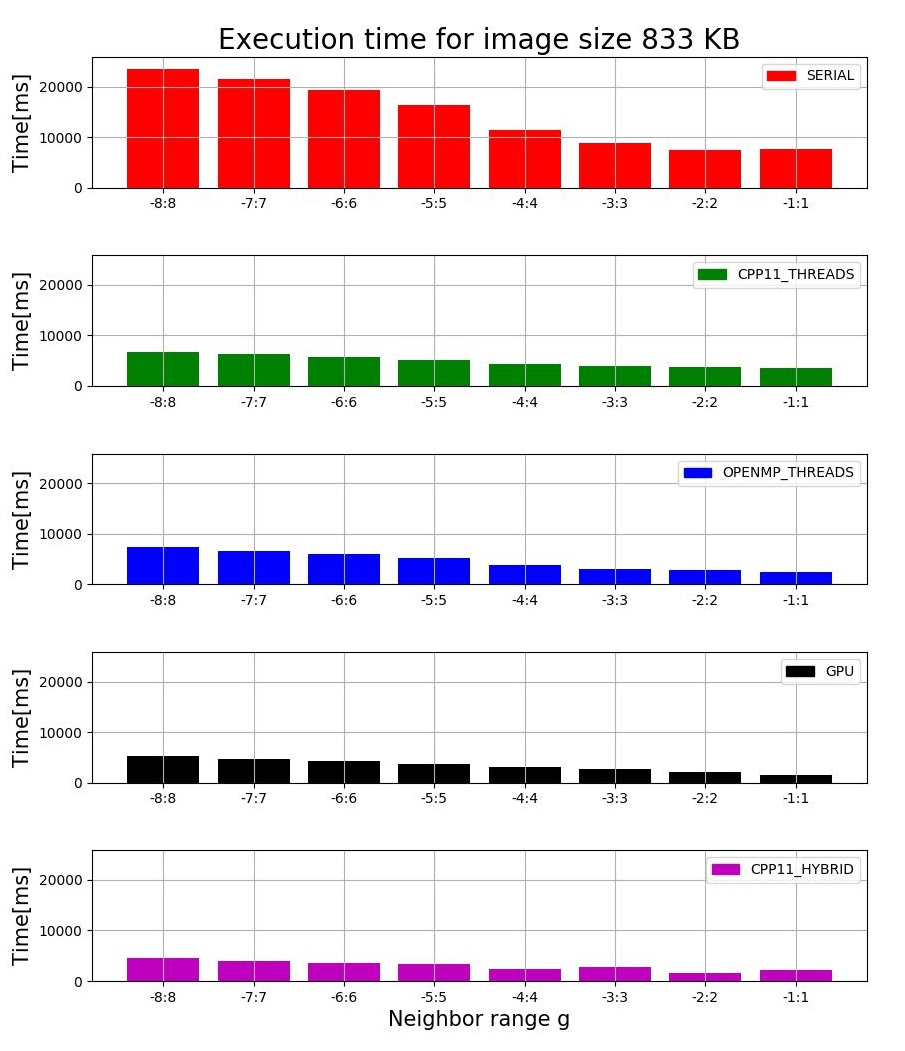
\includegraphics[scale=0.85]{imgs/plot2_pc.png}
\caption{Średni czas przetwarzania zdjęcia w zależności od jego rozmiaru, dla zakresu sąsiedztwa $g\in \langle -8, 8 \rangle$ : $g\in \langle -1, 1 \rangle$}
\label{fig:results_pc_hybrid}
\end{figure}

%------------Analiza wykresów--PC----------------------


%----------------lapek---------------------------------
\clearpage
\subsection{Zestawienie wynikow dla konfiguracji sprzętowej 
Intel i5-6300U 2.4GHz, Intel HD Graphics 520}

\begin{figure}[h]
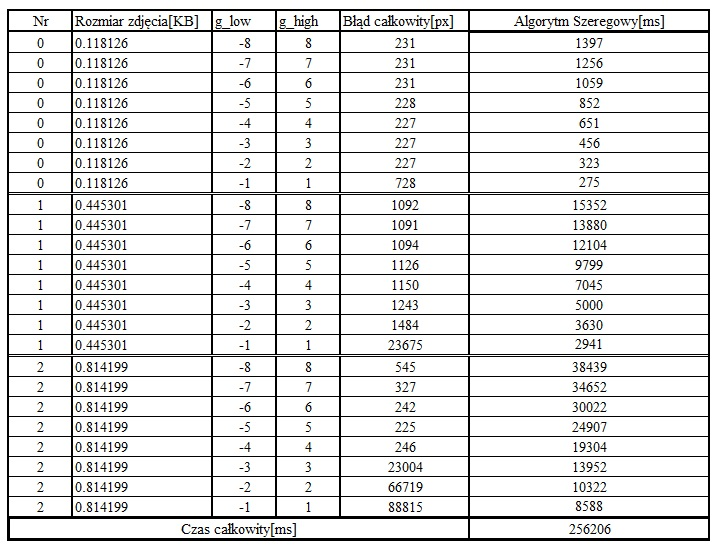
\includegraphics[scale=0.75]{imgs/results_lap_serial}
\caption{Wyniki badań dla algorytmu szeregowego}
\label{fig:results_lap_serial}
\end{figure}

\begin{figure}[h]
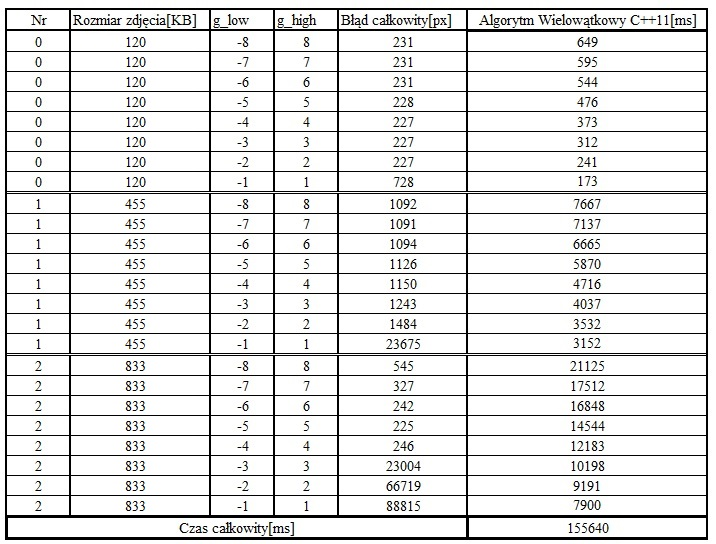
\includegraphics[scale=0.75]{imgs/results_lap_cpp11_threads.jpg}
\caption{Wyniki badań dla algorytmu wielowątkowego korzystającego z C++11}
\label{fig:results_lap_cpp11_threads}
\end{figure}

\begin{figure}[h]
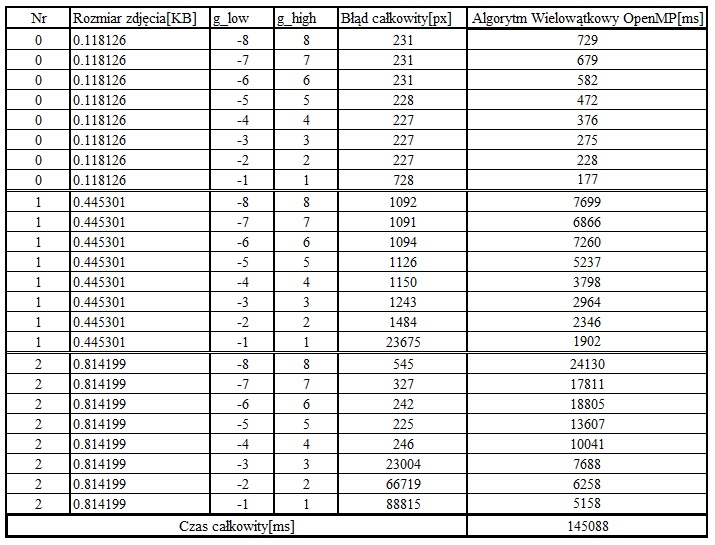
\includegraphics[scale=0.75]{imgs/results_lap_openmp_threads.jpg}
\caption{Wyniki badań dla algorytmu wielowątkowego OpenMP}
\label{fig:results_lap_openmp_threads}
\end{figure}

\begin{figure}[h]
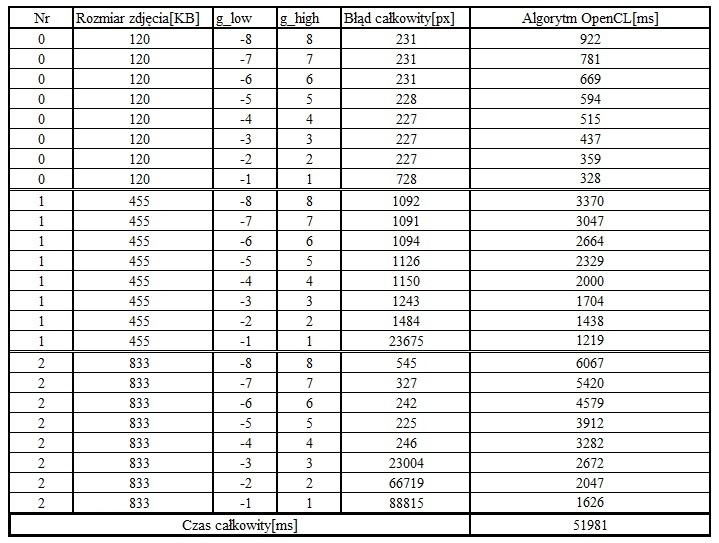
\includegraphics[scale=0.75]{imgs/results_lap_gpu.jpg}
\caption{Wyniki badań dla algorytmu OpenCL}
\label{fig:results_lap_gpu}
\end{figure}

\begin{figure}[h]
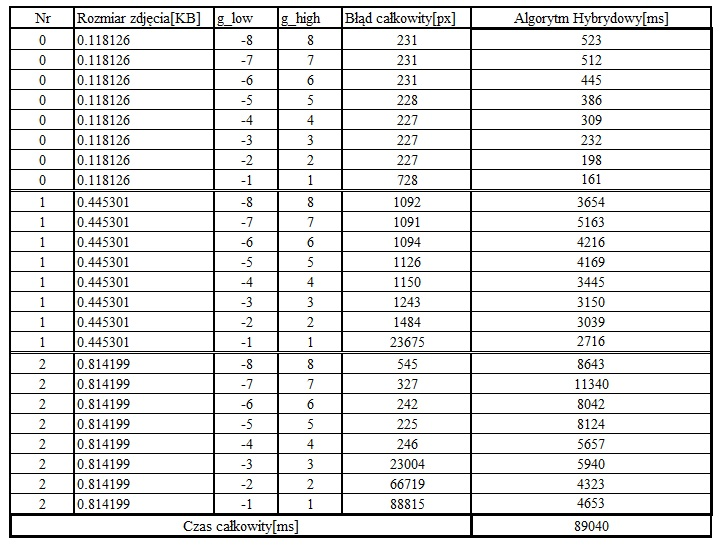
\includegraphics[scale=0.75]{imgs/results_lap_hybrid.jpg}
\caption{Wyniki badań dla algorytmu hybrydowego}
\label{fig:results_lap_hybrid}
\end{figure}

%--------------------------------------------------------------

%wykresy--------------------------------------------------------
\begin{figure}[h]
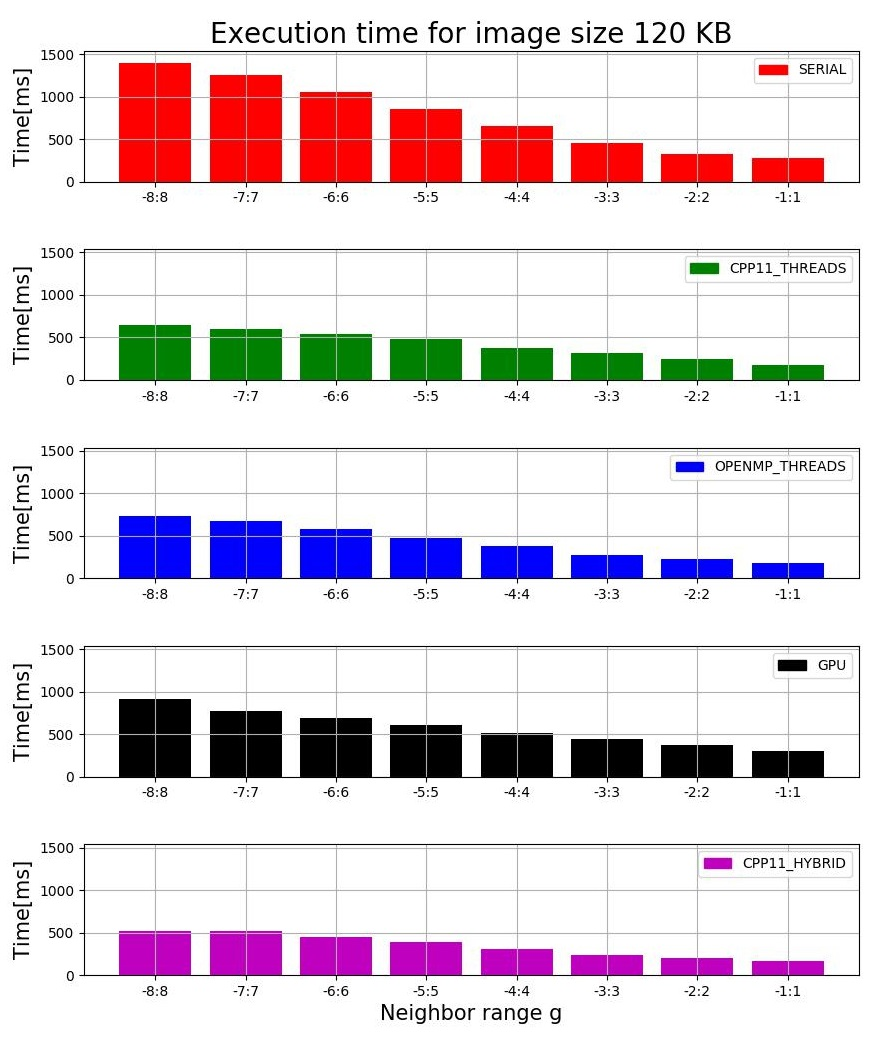
\includegraphics[scale=0.85]{imgs/plot0_lap.png}
\caption*{}
\label{fig:results_lap_hybrid}
\end{figure}

%wykresy
\begin{figure}[h]
\includegraphics[scale=0.85]{imgs/plot7_lap.png}
\caption{Zestawienie czasu wykonania algorytmów dla zdjęcia o rozmiarze 120kB, 
        w zależności od zakresu sąsiedztwa $g\in \langle -8, 8 \rangle$ : $g\in \langle -1, 1 \rangle$ }
\label{fig:results_lap_hybrid}
\end{figure}

%wykresy
\begin{figure}[h]
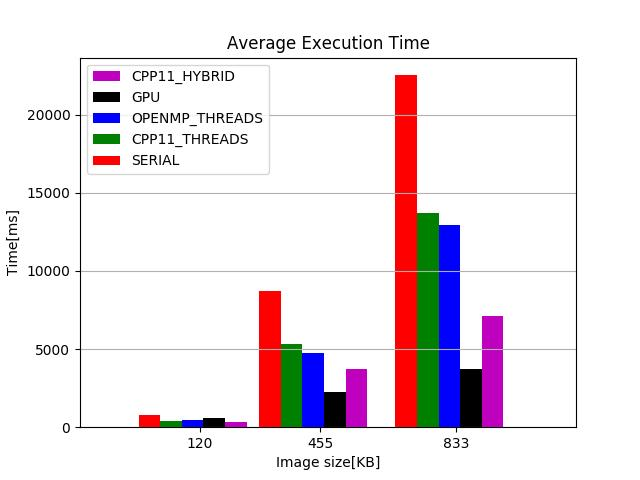
\includegraphics[scale=0.85]{imgs/plot5_lap.png}
\caption*{}
\label{fig:results_lap_hybrid}
\end{figure}

%wykresy
\begin{figure}[h]
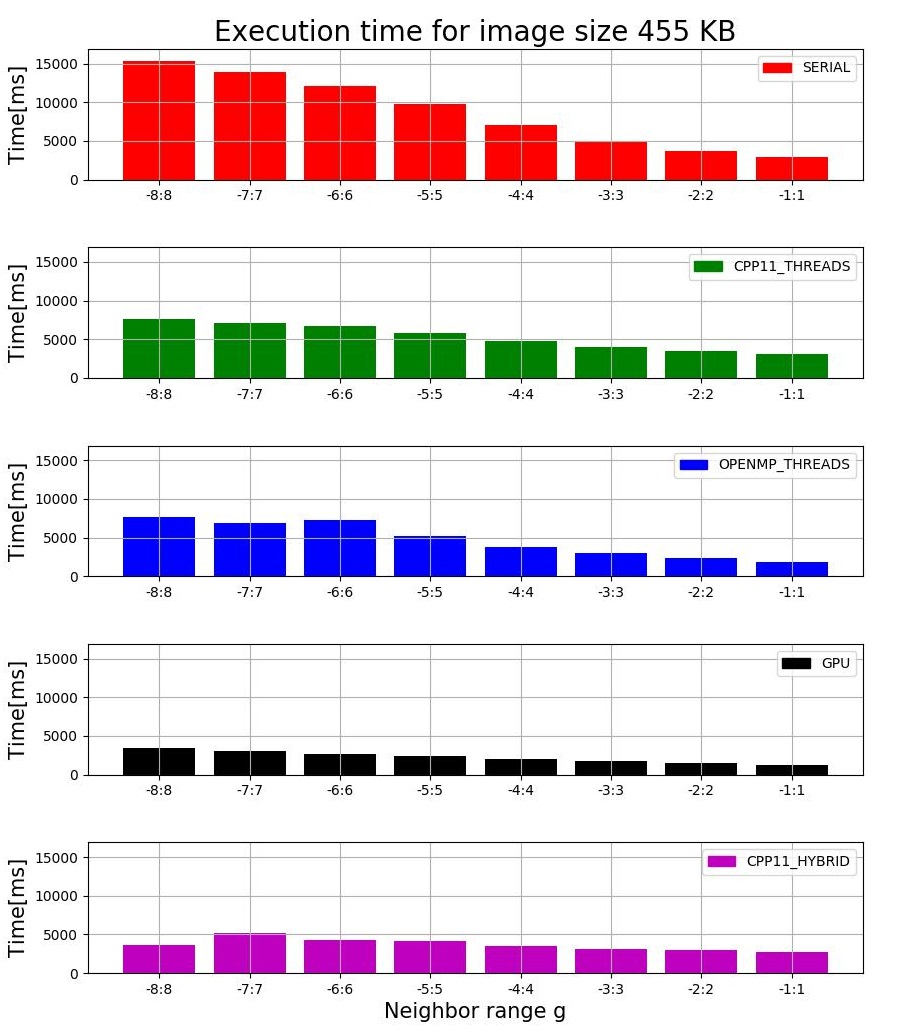
\includegraphics[scale=0.85]{imgs/plot4_lap.png}
\caption{Zestawienie czasu wykonania algorytmów dla zdjęcia o rozmiarze 455kB, 
        w zależności od zakresu sąsiedztwa $g\in \langle -8, 8 \rangle$ : $g\in \langle -1, 1 \rangle$ }
\label{fig:results_lap_hybrid}
\end{figure}

%wykresy
\begin{figure}[h]
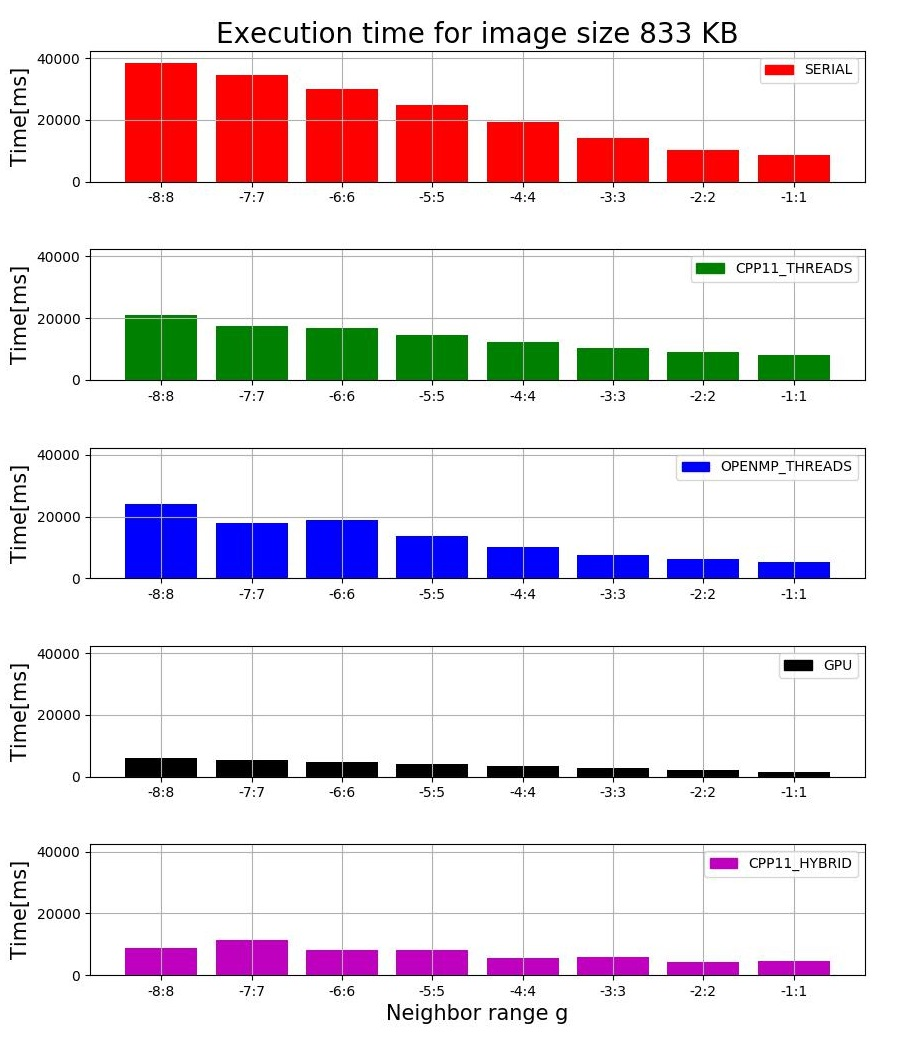
\includegraphics[scale=0.85]{imgs/plot6_lap.png}
\caption*{}
\label{fig:results_lap_hybrid}
\end{figure}

%wykresy
\begin{figure}[h]
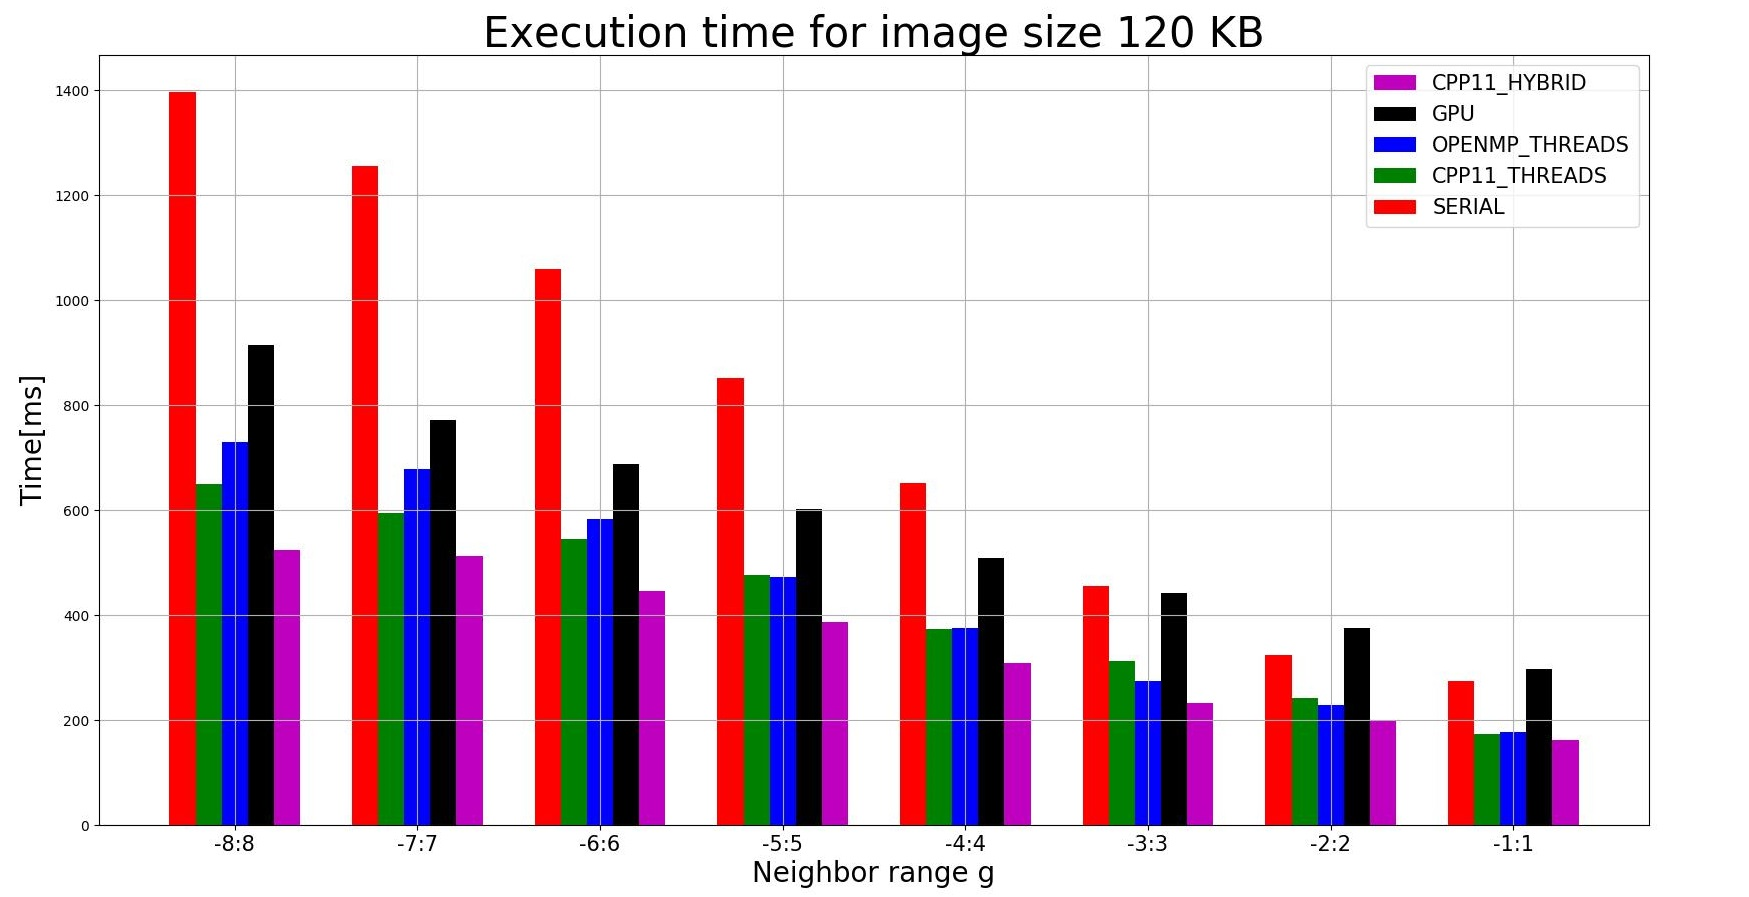
\includegraphics[scale=0.85]{imgs/plot1_lap.png}
\caption{Zestawienie czasu wykonania algorytmów dla zdjęcia o rozmiarze 833kB, 
        w zależności od zakresu sąsiedztwa $g\in \langle -8, 8 \rangle$ : $g\in \langle -1, 1 \rangle$ }
\label{fig:results_lap_hybrid}
\end{figure}

%wykresy
\begin{figure}[h]
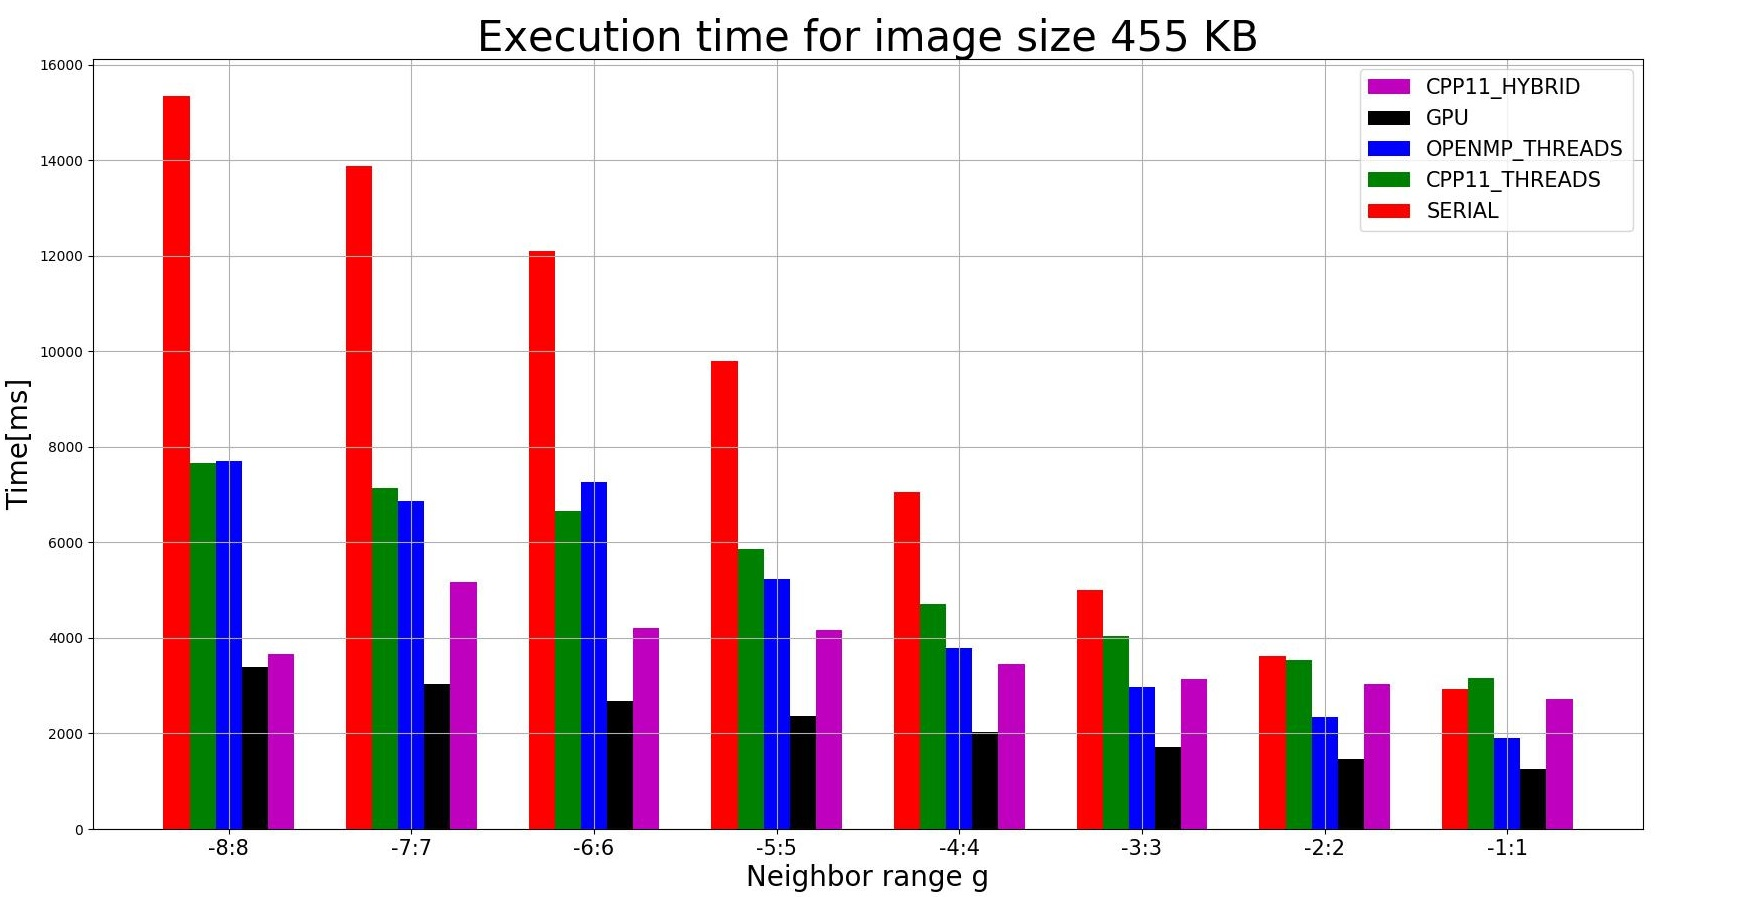
\includegraphics[scale=0.85]{imgs/plot2_lap.png}
\caption{Średni czas przetwarzania zdjęcia w zależności od jego rozmiaru, dla zakresu sąsiedztwa $g\in \langle -8, 8 \rangle$ : $g\in \langle -1, 1 \rangle$}
\label{fig:results_lap_hybrid}
\end{figure}
\clearpage

%------------podsumowanie
\subsection{Analiza wyników badań i porównanie konfiguracji sprzętowych}
\indent Na podsajakdjaskd

\end{document}